\documentclass[12pt,a4paper]{article}

\usepackage[letterpaper]{geometry}
\usepackage{times}
\geometry{top=1.0in, bottom=1.0in, left=1.0in, right=1.0in}


\usepackage{fancyhdr}
\pagestyle{fancy}
\lhead{} 
\rhead{}
\chead{} 
\lfoot{} 
\cfoot{} 
\rfoot{} 
\renewcommand{\headrulewidth}{0pt} 
\renewcommand{\footrulewidth}{0pt} 
%To make sure we actually have header 0.5in away from top edge
%12pt is one-sixth of an inch. Subtract this from 0.5in to get headsep value
\setlength\headsep{0.333in}

\usepackage{fontspec}
\setmainfont{Times New Roman}

\usepackage{graphicx}



% =============================
\begin{document}

\linespread{2}

% =============================

%NOTE: cover page
\begin{center}
\vspace*{0.7in}
%\includegraphics[width=0.55\textwidth]{./pot}\\[1cm]    
\vspace*{0.7in}

%\textsc{\Large Major Research Paper}\\[0.5cm]


% Title


% Author and supervisor

\begin{center} 


\includegraphics[height=3cm]{picture/umjiLogo}


{
\linespread{2}
\LARGE
\textsc{VG100 Introduction To Engineering} \\
}
{
\Large
\textsc{Project 1 Bridge Crane} \\
}


\vspace*{0.6in}

\textsc{\large Group 3 Trinity}\\

\vspace*{0.2in}


\begin{tabular}{cc}
{\fontspec{Hei}\selectfont 谢舒翔} & Shuxiang \textsc{Xie} \\
{\fontspec{Hei}\selectfont 郭成彰} & Chengzhang \textsc{Guo} \\
{\fontspec{Hei}\selectfont 麻珂睿} & Kerui \textsc{Ma} \\
{\fontspec{Hei}\selectfont 王韧} & Ren \textsc{Wang} \\
{\fontspec{Hei}\selectfont 朱波颖} & Boying \textsc{Zhu} \\
\end{tabular}


\vspace*{0.5in}

\begin{tabular}{cc}
Professor & Yanfeng \textsc{Shen} \\
Professor & Cynthia \textsc{Vagnetti} 
\end{tabular}


\vspace*{0.7in}

{\today}


\end{center}



% Bottom of the page
\end{center}
\newpage
% NOTE: end of cover page

% =============================

\rhead{\textsc{Group 3}}
\lhead{
\includegraphics[height=1cm]{picture/umjiLogo}}

\tableofcontents
\newpage

\section{Introduction}

\subsection{About Us and Campus}


\begin{figure}[htbp]
\centering

\includegraphics[height=8cm]{picture/teamMember}
  \caption{Our team \label{fig:teamMember}}
\end{figure}

We are TRINITY (Figure \ref{fig:teamMember}), a team of freshmen from University of
Michigan-Shanghai Jiao Tong University Joint Institute (UM-SJTU JI), which is
located in the campus of Shanghai Jiao Tong University (Figure
\ref{fig:campus}). People in the photo are Xie Shuxiang, Zhu Boying, Ma Kerui,
Wang Ren and Guo Chengzhang, and our group leader is Xie Shuxiang. Joint
Institute is well-known for its unique way of helping students develop the
ability of cooperation and innovation. As a result, students here have various
projects and activities to attend to broaden their horizons.  


\begin{figure}[htbp]
\centering
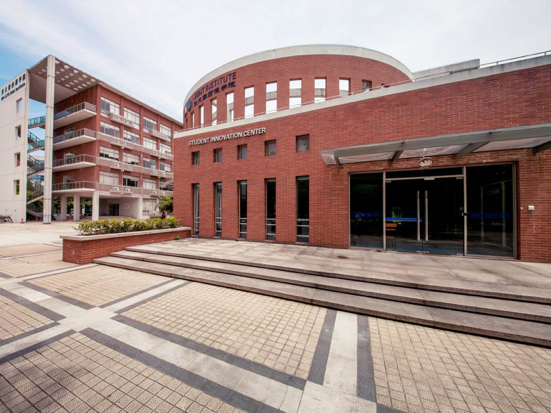
\includegraphics[height=5cm]{figure/campus}
  \caption{\label{fig:campus}}
\end{figure}

\subsection{Course and Project Information}


VG100 is a course about Introduction to Engineering. It is a mandatory course
for all freshmen in JI. According to Professor Shen Yanfeng, the course not only
convey fundamental knowledge of engineering, but also help students learn how to
solve a realistic problem. Besides, the technical communication part strengthens
students’ ability of taking part in teamwork, which is of great importance for
engineers.  

The first project students should accomplish in VG100 is to make a bridge-crane
system. It should be able to allow a cart to pull a cup of water up, travel
forward on the bridge to the other side, and put down the cup of water on the
designated place (Figure \ref{fig:structureOfP1}).  

\begin{figure}[htbp]
\centering
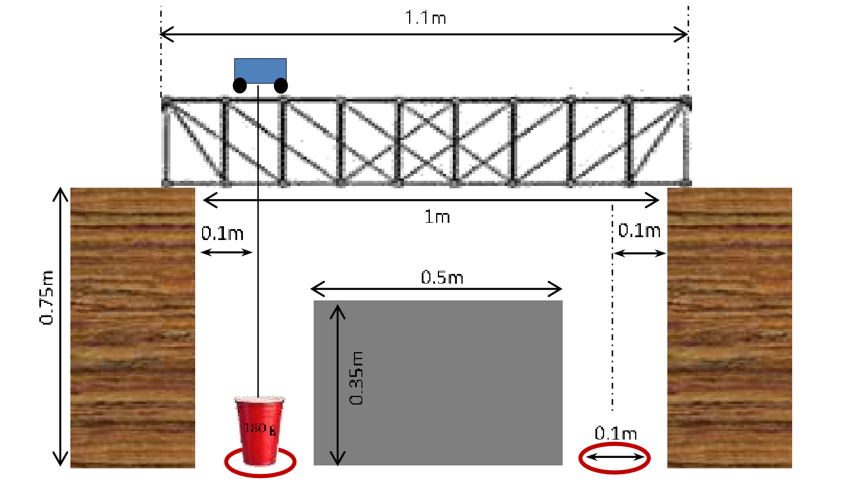
\includegraphics[height=5cm]{figure/structureOfP1}
\caption{\label{fig:structureOfP1}}
\end{figure}

The following list from the professor shows the specific requirement of Project 1.
Mechanism: Any method that can achieve the above task will be acceptable.
Breaking any of these rules will result in failing project 1.  
Bridge length:  >= 1.1m 
Bridge width:  <= 0.2 m 
Bridge Material: printing paper (80g size A4) and non-toxic, white wood glue
(brand: LongMa). Any additional material violates the rule!  
Maximum Mass of the bridge: 200g 
Maximum length of the cart: 0.1 m 
Power Supply: Maximum two portable Power Supply (for each battery Voltage ≤ 12V) 
Motor specifications: < 12V.  
Central Control Circuit: Arduino series (Required for Programming \& Can Be Omitted)

\subsection{Race Performance}
(This part will be completed later)

 % introduction
\input{part/designOverview} % design overview
\section{Materials \& Tools}
% images
\newcommand{\beginMyTabular}{
    \begin{center}
    \begin{tabular}{p{0.4cm}p{5cm}p{5cm}rr}
    \hline
    No. & Item & Specification & Quantity & Price(Yuan) \\
    \hline
}
\newcommand{\MyTabularEnd}{
    \hline
    \end{tabular}
    \end{center}
}
% counter
\newcounter{matcnt}
\setcounter{matcnt}{0}
\newcommand{\CounterOfM}{
    \stepcounter{matcnt}\arabic{matcnt}
}
% CounterOfM means the counter of materials
%
\newcounter{figcnt}
\setcounter{figcnt}{0}
\newcommand{\CounterOfF}{
    \stepcounter{figcnt}\arabic{figcnt}
}
\newcommand{\CounterOfFa}[1]{
    \raisebox{#1cm}{
        \fbox{\small \CounterOfF} \hspace{0.3cm}
    }
    \nolinebreak[3]
}
\newcommand{\MPGx}[3]{
    \CounterOfFa{#1}
	\begin{minipage}{0.2\textwidth}
    \centering    
    \includegraphics[height=#2cm]{picture/material/#3}
    \end{minipage}
}
\newcommand{\MPGxA}[3]{
    \CounterOfFa{#1}
	\begin{minipage}{0.1\textwidth}
    \centering    
    \includegraphics[height=#2cm]{picture/material/#3}
    \end{minipage}
}
%% ====================================================
%% ====================================================
%% ====================================================
\newcommand{\HPRx}{1.4}
\newcommand{\HPx}{2}
\newcommand{\MyWidthFirstLine}{3.3cm}

%\begin{flushleft}
%\begin{tabular}{p{\MyWidthFirstLine}p{\MyWidthFirstLine}p{\MyWidthFirstLine}p{\MyWidthFirstLine}}
%\end{tabular}
%\end{flushleft}
%
\begin{center}
\begin{tabular}{lll}
\MPGxA{\HPRx}{\HPx}{a4paper} & \MPGxA{\HPRx}{\HPx}{whiteglue} & \MPGxA{\HPRx}{\HPx}{papercutter} \\
\MPGxA{\HPRx}{\HPx}{brush} & \MPGx{\HPRx}{\HPx}{woodstick} & \MPGx{\HPRx}{\HPx}{scissor} \\
\MPGx{\HPRx}{\HPx}{arduino} & \MPGx{\HPRx}{\HPx}{standN20} & \MPGx{\HPRx}{\HPx}{moterN20} \\
\MPGx{\HPRx}{\HPx}{wheelrubber} & \MPGx{\HPRx}{\HPx}{servo360} & \MPGx{\HPRx}{\HPx}{batteryPlane} \\
\MPGx{\HPRx}{\HPx}{batteryBreeze} & \MPGx{\HPRx}{\HPx}{switch} & \MPGx{\HPRx}{\HPx}{pcbBoard} \\  
\MPGx{\HPRx}{\HPx}{tapeThick} & \MPGx{\HPRx}{\HPx}{stringYoYo} & \MPGx{\HPRx}{\HPx}{m3} \\ 
\MPGx{\HPRx}{\HPx}{m2} & \MPGx{\HPRx}{\HPx}{car} \\
\end{tabular}
%
\end{center}
%
\subsection{Bridge}
\subsubsection{Materials}
% tables
\beginMyTabular
\CounterOfM & A4 paper & Double A 80 g  A4 paper  & 10 & 29.8 \\
\CounterOfM & Long Ma White Glue & 400 g & 5 & 67.5 \\
\MyTabularEnd

\subsubsection{Tools}

% images

% tables
\beginMyTabular
\CounterOfM & Huanmei Paper Cutter & & 1 & 34.8 \\
\CounterOfM & Brush & 5 mm width & 5 & 10.6 \\
\CounterOfM & Wood Stick & 5 mm $\times $ 5 mm & 10 & 4 \\ 
\CounterOfM & Qixing Scissor &  & 1 & 4.6 \\ 
\MyTabularEnd

% ======================================

\subsection{Cart}
\subsubsection{Materials}

% tables
\beginMyTabular
\CounterOfM & XTWduino UNO Arduino & V3.0 ATMEGA328P & 1 & 25\\
\CounterOfM & N20 stand &  & 1 & 0.99\\
\CounterOfM & N20 Moter & 12V 150 rpm & 1 & 19.80 \\
\CounterOfM & Rubber Wheel & Diameter: 43 mm  &  2  & 5.4 \\
\CounterOfM & TowerPro 360 Degree servo & MG996R  & 1 & 38\\
\CounterOfM & Plane model Battery & 7.4 &1  & 37.8\\
\CounterOfM & Breeze 2s/3s Battery & 11.1V 500mAh& 1& 31\\
\CounterOfM & Bridge-shaped  Switch & &1 &1.6 \\
\CounterOfM & PCB Hole Board & 9 * 15 cm Gap 2.54 mm & 1 & 6 \\
\CounterOfM & 3M Thick Plastic tape & 1 cm Width & 1 & 7 \\
\CounterOfM & Audi YoYo String & & 1 & 7.9 \\
\MyTabularEnd

\subsubsection{Tools}
% images

% tables
\beginMyTabular
\CounterOfM & M3 screws and nuts  & 3 mm & 2 & 0.75 \\
\CounterOfM & M2 screws and nuts & 2 mm &  4 & 0.65  \\
\CounterOfM & Model cart &  & 1 & 28 \\
\MyTabularEnd % material
\section{Instructions}
\subsection{Bridge}
\subsection{Cart} % instruction
\section{Improvements} % improvement
\section{Appendix} % appendix reference

\end{document}